\documentclass[a4paper,14pt]{extarticle}

\usepackage[utf8x]{inputenc}
\usepackage[T1]{fontenc}
\usepackage[russian]{babel}
\usepackage{hyperref}
\usepackage{indentfirst}
\usepackage{here}
\usepackage{array}
\usepackage{graphicx}
\usepackage{caption}
\usepackage{subcaption}
\usepackage{chngcntr}
\usepackage{amsmath}
\usepackage{amssymb}
\usepackage[left=2cm,right=2cm,top=2cm,bottom=2cm,bindingoffset=0cm]{geometry}
\usepackage{multicol}
\usepackage{multirow}
\usepackage{titlesec}
\usepackage{listings}
\usepackage{color}
\usepackage{enumitem}
\usepackage{cmap}
\usepackage{underscore}

\definecolor{green}{rgb}{0,0.6,0}
\definecolor{gray}{rgb}{0.5,0.5,0.5}
\definecolor{purple}{rgb}{0.58,0,0.82}

\lstdefinelanguage{none}{}

\lstset{
	language={Java},
	inputpath={../generator/src/main/java/com/vaddya/hotelbooking},
	backgroundcolor=\color{white},
	commentstyle=\color{green},
	keywordstyle=\color{blue},
	numberstyle=\scriptsize\color{gray},
	stringstyle=\color{purple},
	basicstyle=\ttfamily\small,
	breakatwhitespace=false,
	breaklines=true,
	captionpos=b,
	keepspaces=true,
	numbers=left,
	numbersep=5pt,
	showspaces=false,
	showstringspaces=false,
	showtabs=false,
	tabsize=4,
	texcl=true,
	extendedchars=false,
	frame=single,
	morekeywords={IF, BIGSERIAL, SERIAL, TEXT, BIGINT, MONEY, BOOLEAN, REFERENCES}
}

\renewcommand{\le}{\ensuremath{\leqslant}}
\renewcommand{\leq}{\ensuremath{\leqslant}}
\renewcommand{\ge}{\ensuremath{\geqslant}}
\renewcommand{\geq}{\ensuremath{\geqslant}}
\renewcommand{\epsilon}{\ensuremath{\varepsilon}}
\renewcommand{\phi}{\ensuremath{\varphi}}
\renewcommand{\thefigure}{\arabic{figure}}
\newcommand{\code}[1]{\texttt{#1}}
\newcommand{\caret}{\^{}}

\titleformat*{\section}{\large\bfseries} 
\titleformat*{\subsection}{\normalsize\bfseries} 
\titleformat*{\subsubsection}{\normalsize\bfseries} 
\titleformat*{\paragraph}{\normalsize\bfseries} 
\titleformat*{\subparagraph}{\normalsize\bfseries} 

\counterwithin{figure}{section}
\counterwithin{equation}{section}
\counterwithin{table}{section}
\newcommand{\sign}[1][5cm]{\makebox[#1]{\hrulefill}}
\newcommand{\equipollence}{\quad\Leftrightarrow\quad}
\newcommand{\no}[1]{\overline{#1}}
\graphicspath{{../pics/}}
\captionsetup{justification=centering,margin=1cm}
\def\arraystretch{1.3}
\setlength\parindent{5ex}
\titlelabel{\thetitle.\quad}

\setitemize{topsep=0.5em, itemsep=0em}
\setenumerate{topsep=0.5em, itemsep=0em}

\begin{document}

\begin{titlepage}
\begin{center}
	Санкт-Петербургский Политехнический Университет Петра Великого\\[0.3cm]
	Институт компьютерных наук и технологий \\[0.3cm]
	Кафедра компьютерных систем и программных технологий\\[4cm]
	
	\textbf{ОТЧЕТ}\\ 
	\textbf{по лабораторной работе}\\[0.5cm]
	\textbf{<<Разработка структуры базы данных>>}\\[0.1cm]
	Базы данных\\[3.0cm]
\end{center}

\begin{flushright}
	\begin{minipage}{0.45\textwidth}
		\textbf{Работу выполнил студент}\\[3mm]
		группа 43501/3 \hfill Дьячков В.В.\\[5mm]
		\textbf{Работу принял преподаватель}\\[5mm]
		\sign[3cm] \hfill Мяснов А.В. \\[5mm]
	\end{minipage}
\end{flushright}

\vfill

\begin{center}
	Санкт-Петербург\\[0.3cm]
	\the\year
\end{center}
\end{titlepage}

\addtocounter{page}{1}

\tableofcontents
\newpage

\section{Цель работы}

Познакомиться с основами проектирования схемы БД, способами организации данных в SQL-БД.

\section{Программа работы}

\begin{enumerate}
	\item Создание проекта для работы в GitLab.
	\item Выбор задания (предметной области), описание набора данных и требований к хранимым данным в свободном формате в Wiki своего проекта в GitLab.
	\item Формирование в свободном формате (предпочтительно в виде графической схемы) схемы БД, соответствующей заданию. Должно получиться не менее 7 таблиц.
	\item Согласование с преподавателем схемы БД. Обоснование принятых решений и соответствия требованиям выбранного задания. 
	\item Выкладывание схемы БД в свой проект в GitLab.
	\item Демонстрация результатов преподавателю.
\end{enumerate}

\section{Выполнение работы}


\subsection{Выбор предметной области}

В качестве предметной области была выбрана система онлайн-бронирования отелей. База данных такой системы хранит информацию об отелях, доступных в них номерах и предоставляемых удобствах, ценах на определенные даты, бронированиях и отзывах.

\subsection{Описание таблиц}

\begin{itemize}
	\item \code{Price} -- хранит информацию о цене \code{price} в период с \code{from} по \code{to} за сутки в номере с типом \code{room_type_id} (например, с 01.10.2018 по 31.10.2018 сутки проживания в номере с типом 123 стоят 4567 рублей).
	
	\item \code{RoomType} -- хранит информацию о типе номера \code{type} в отеле \code{hotel_id}: вместимость \code{capacity} и описание \code{description} (например, двухместный <<номер для некурящих с 2 кроватями размера king-size>> в отеле <<Гранд Будапешт>>).
	
	\item \code{RoomFacility} -- дополнительная таблица для создания отношения многие ко многим между типом номера \code{room_type_id} и предоставляемым удобством \code{facility_id}.
	
	\item \code{Facility} -- хранит информацию о предоставляемом в номере удобстве \code{name} (например, Wi-Fi).
	
	\item \code{Hotel} -- хранит информацию об отеле \code{name}: внешний ключ на условия размещения \code{house_rules_id}, адрес \code{address}, количество звезд \code{stars} и текстовое описание \code{description}.
	
	\item \code{Room} -- хранит информацию о конкретных номерах с типом \code{room_type_id} (например, номер <<№123>> c типом <<номер для некурящих с 2 кроватями размера king-size>>).
	
	\item \code{Reservation} -- хранит информацию о бронировании номера \code{room_id} пользователем \code{user_id} с \code{from} по \code{to}, итоговой цене проживания \code{price} и информацию о совершении платежа \code{is_paid}.
	
	\item \code{Cancellation} -- хранит информацию о статусе \code{status} отмены бронирования \code{reservation_id}.
	
	\item \code{HouseRules} -- хранит информацию о правилах проживания в отеле: время заезда \code{checkin_from} и отъезда \code{checkout_until} (например, заезд после 15:00, отъезд до 12:00), политика отмены бронирования и возврата средств \code{cancellation_policy} (например, предоплата не возвращается при отмене бронирования меньше за сутки).
	
	\item \code{Review} -- хранит плюсы \code{advantages}, минусы \code{disadvantages} и итоговый рейтинг \code{rating} о проживании \code{reservation_id} (например, плюсы: вкусный завтрак, минусы: холодно, итоговый рейтинг: 3 из 5).
	
	\item \code{Guest} -- хранит имя гостя \code{name} и информацию о том, является ли он ребенком \code{is_child}, указанную при бронировании \code{reservation_id}.
	
	\item \code{User} -- хранит имя \code{name}, электронную почту \code{email}, hash от пароля \code{password_hash} и номер телефона \code{phone_number} пользователя.
\end{itemize}

\subsection{Структура базы данных}

\begin{figure}[H]
	\centering
	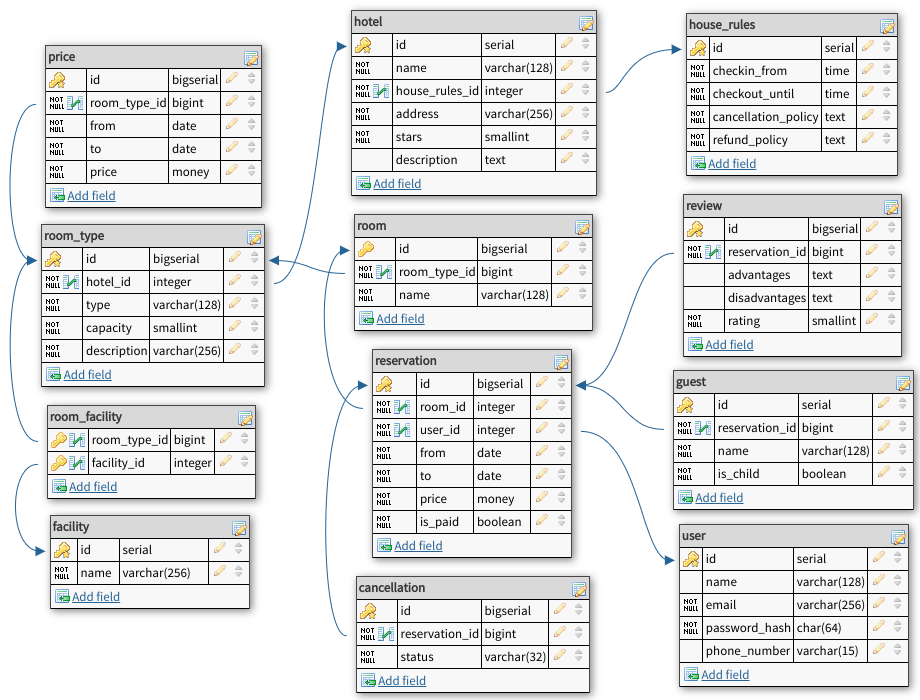
\includegraphics[width=\linewidth]{../../scheme}
\end{figure}

\section{Выводы}

В ходе выполнения данной работы была спроектирована и согласована с преподавателем база данных для системы онлайн-бронирования отелей. Было выделено несколько основные сущностей, таких как отель, номер, бронирование и пользователь, а также множество вспомогательных таблиц для хранения информации о предоставляемых удобствах, условиях размещения и отзывах.

\end{document}
